\pdfminorversion=4
\documentclass[aspectratio=169]{beamer}

\mode<presentation>
{
  \usetheme{default}
  \usecolortheme{default}
  \usefonttheme{default}
  \setbeamertemplate{navigation symbols}{}
  \setbeamertemplate{caption}[numbered]
  \setbeamertemplate{footline}[frame number]  % or "page number"
  \setbeamercolor{frametitle}{fg=white}
  \setbeamercolor{footline}{fg=black}
} 

\usepackage[english]{babel}
\usepackage[utf8x]{inputenc}
\usepackage{tikz}
\usepackage{courier}
\usepackage{array}
\usepackage{bold-extra}
\usepackage{minted}
\usepackage[thicklines]{cancel}
\usepackage{fancyvrb}

\xdefinecolor{dianablue}{rgb}{0.18,0.24,0.31}
\xdefinecolor{darkblue}{rgb}{0.1,0.1,0.7}
\xdefinecolor{darkgreen}{rgb}{0,0.5,0}
\xdefinecolor{darkgrey}{rgb}{0.35,0.35,0.35}
\xdefinecolor{darkorange}{rgb}{0.8,0.5,0}
\xdefinecolor{darkred}{rgb}{0.7,0,0}
\definecolor{darkgreen}{rgb}{0,0.6,0}
\definecolor{mauve}{rgb}{0.58,0,0.82}

\title[2018-08-21-cmsblueprint-querysystem]{Query-based analysis: how to get there?}
\author{Jim Pivarski}
\institute{Princeton University -- DIANA-HEP}
\date{August 21, 2018}

\usetikzlibrary{shapes.callouts}

\begin{document}

\logo{\pgfputat{\pgfxy(0.11, 7.4)}{\pgfbox[right,base]{\tikz{\filldraw[fill=dianablue, draw=none] (0 cm, 0 cm) rectangle (50 cm, 1 cm);}\mbox{\hspace{-8 cm}
\includegraphics[height=1 cm]{princeton-logo-long.png}
\includegraphics[height=1 cm]{diana-hep-logo-long.png}}}}}

\begin{frame}
  \titlepage
\end{frame}

\logo{\pgfputat{\pgfxy(0.11, 7.4)}{\pgfbox[right,base]{\tikz{\filldraw[fill=dianablue, draw=none] (0 cm, 0 cm) rectangle (50 cm, 1 cm);}\mbox{\hspace{-8 cm}
\includegraphics[height=1 cm]{princeton-logo.png}
\includegraphics[height=1 cm]{diana-hep-logo.png}}}}}

% Uncomment these lines for an automatically generated outline.
%\begin{frame}{Outline}
%  \tableofcontents
%\end{frame}

% START START START START START START START START START START START START START

\begin{frame}{Query-based analysis}
\large
\vspace{0.5 cm}
\textcolor{darkorange}{\bf Different performance characteristics $\to$ sociological consequences}

\vspace{1 cm}
\begin{columns}
\column{0.3\linewidth}
\underline{\Large Batch job}

\vspace{0.2 cm}
Long time to compute one complex function
\column{0.3\linewidth}
\underline{\Large Query}

\vspace{0.2 cm}
Short time to compute each simple function
\end{columns}

\vspace{1 cm}
\begin{uncoverenv}<2->
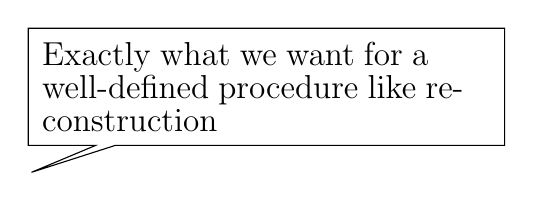
\begin{tikzpicture}[>=latex]
\node[rectangle callout, draw, inner sep=5 pt, callout relative pointer={(200:1 cm)}, text width=0.47\linewidth] {\large Exactly what we want for a well-defined procedure like reconstruction};
\end{tikzpicture} \hfill 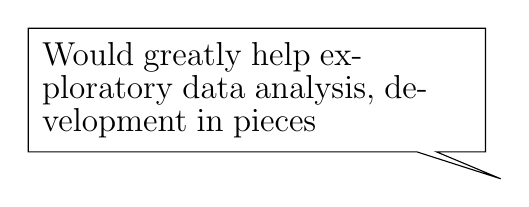
\begin{tikzpicture}[>=latex]
\node[rectangle callout, draw, inner sep=5 pt, callout relative pointer={(-200:-1 cm)}, text width=0.45\linewidth] {\large Would greatly help exploratory data analysis, development in pieces};
\end{tikzpicture}
\end{uncoverenv}
\end{frame}

\begin{frame}{Different ``performance characteristics''}
\large
\vspace{0.5 cm}
Not promising a miracle--- more computation in less time--- but scaling that fits many short jobs (``queries'') instead of few big jobs.

\vspace{0.5 cm}
\uncover<2->{\textcolor{darkblue}{\underline{What needs to change:}}}

\vspace{0.2 cm}
\begin{itemize}
\item<3-> Startup time must be below a human timescale, like 100~ms. \textcolor{gray}{Workers must be ready and waiting, not launched.}
\item<4-> Input data (which will always be large, like TB/query) must be cached on the workers. \textcolor{gray}{Work must be performed by the worker who already has the relevant fragment in cache.}
\item<5-> Loading data from cache to the user function must not dominate over the user function. \textcolor{gray}{This is what I've been focusing on.}
\item<6-> Output data must be small, like MB/query--- GB/query at most.
\end{itemize}
\end{frame}

\begin{frame}{Query services in the wild}
\hfill 
\includegraphics[height=1.5 cm]{google-bigquery-logo.png}

\vspace{-1.25 cm}
Google BigQuery is a public-facing SQL processor that runs my \\ 2~TB queries in 30~seconds.

\vspace{0.5 cm}
\hfill \uncover<2->{
\includegraphics[height=1 cm]{binder-logo.pdf}}

\vspace{-1.1 cm}
\uncover<2->{Binder is a free service that runs any Jupyter Notebook you have \\ on a GitHub repository.}

\vspace{0.25 cm}
\begin{uncoverenv}<3->
\textcolor{gray}{\small
Search on GitHub: {\tt\scriptsize binder in:path path:/binder} yields \textcolor{black}{9,754} Binder setup files. \\
Search on GitHub: {\tt\scriptsize https://mybinder.org/badge.svg language:Markdown} yields \textcolor{black}{3,835} badges.}
\end{uncoverenv}

\begin{uncoverenv}<4->
\begin{columns}
\column{0.35\linewidth}
\small
$\sim$200 notebooks running at a time, served by 5 machines

\vspace{0.25 cm}
\scriptsize Tim Head: ``The trick is to \mbox{oversubscribe\hspace{-0.5 cm}} the CPU massively, turns out humans take a long time to read what a notebook computed for them.''

\normalsize
\vspace{0.25 cm}
\centering 1 user $\neq$ 1 CPU!

\column{0.6\linewidth}
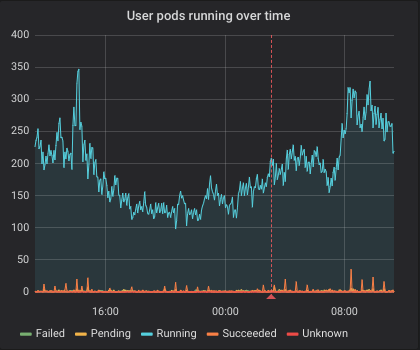
\includegraphics[height=3 cm]{binder-notebooks-running.png}\mbox{ }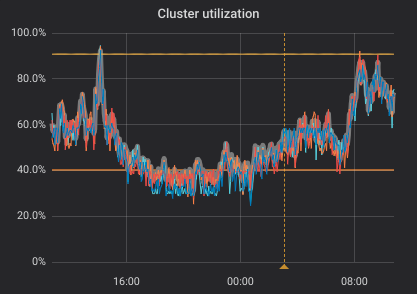
\includegraphics[height=3 cm]{binder-utilization.png}
\end{columns}
\end{uncoverenv}
\end{frame}





\end{document}
